\section{问题重述与问题分析}

\subsection{问题背景}

微网是一种可就地消纳分布式光伏、减少并网冲击的小型发用电系统。与外部电网并网运行时，其核心经济行为是``低买高卖''：在外网电价较低或光伏出力富余时为储能设备充电，在电价较高时放电供电，从而在满足小区负载的前提下压低购电费用。

题目数据构成一条逐层放开的``信息链''：附件 1 给出单日的电价、小区负载与光伏预测功率，附件 2 至附件 4 分别给出全年的负载与光伏实测值、四个发布时点的光伏预报、全年实时电价，附件 5 为结果填报模板。储能设备的物理边界为：容量上限 12000 kWh、最大充放电功率 5000 kW、运行区间 1200$\sim$10800 kWh、充放电效率各 90\%，2025 年 1 月 1 日 0:00 的初始储电量为 6000 kWh。二者构成四问共用的输入与约束。

\subsection{问题提出}

四问共享同一物理场景与同一套储能边界，差别只在三点：决策时点能获得哪些信息、决策变量有多少自由度、以及费用如何结算。按这一理解，四问的建模任务可概括如下。

\textbf{问题一（确定性单日调度）：}电价、负载与光伏预测全部已知，需要在日初一次性给出全天的计划购电量与充放电轨迹，使全天购电费用最小，并满足逐时段电力平衡与日初、日末储电量相等的要求。该问本质上是一个以购电费为目标、以储电量为唯一耦合变量的确定性线性规划，为后续各问提供调度内核与费用基准。

\textbf{问题二（负荷与光伏不确定下的日前决策）：}电价规律仍已知，但负载与光伏在日初尚未揭晓，只能使用此前的历史实测值；计划量一旦定下不得更改，实际出现缺口时只能以 5 倍电价紧急购电。因此该问是含预测误差的随机优化：需要分别预测当天 144 个时段的负荷与光伏，用预测误差的分布刻画不确定性，并把跨日储电量的价值写进单日模型，防止模型逐日透支储能。

\textbf{问题三（光伏预报更新下的日内滚动决策）：}在问题二的基础上，日初之外还可获得 6:00、12:00、18:00 三次更新的未来光伏预报，允许修改尚未执行时段的购电计划；上调与下调分别按 1.5 倍与 50\% 电价结算。该问由``一次决策''变为``多次滚动决策''，需要处理已执行时段的不可回溯性、剩余时域的重新优化以及调整费用的线性化，并回答引入哪些时点的预报才值得。

\textbf{问题四（波动电价下的重算）：}把固定的日内电价换成逐日变化的实时电价，要求在电价同样只能预测的前提下重算问题二与问题三，并区分``可实施的现实策略''与``假想全知的价格完全信息基准''，以量化价格预测误差造成的经济损失。

\subsection{问题分析}

四问的关系是``同一内核、逐层加难''，因此本文不为每一问另写一套模型，而是先抽出公共调度内核——逐时段电力平衡、储能状态递推、充放电互斥与储电量边界——再逐问叠加预测、场景、滚动与价格波动，形成统一的``预测---场景---优化---结算''框架。

其中，贯穿全文各类调度场景的电力平衡关系为

\begin{equation}
  P(t) + G(t) + H(t) + D(t) = L(t) + C(t) + W(t).
  \label{eq:unified_power_balance}
\end{equation}

式中，光伏可利用电量 $P(t)$、计划购电量 $G(t)$、紧急购电量 $H(t)$ 与储能放电量 $D(t)$ 共同构成时段供给；负荷电量 $L(t)$、储能充电量 $C(t)$ 与弃光（或无法消纳的富余）电量 $W(t)$ 共同构成时段去向。问题一中不发生紧急购电，故 $H(t)=0$；问题三、问题四的滚动重优化中，以调整后购电量 $A^{(\tau)}(t)$ 替代 $G(t)$。因此，各问虽在信息边界和购电机制上不同，均可由式~\eqref{eq:unified_power_balance} 保证逐时段电量守恒，关系如图~\ref{fig:unified_power_balance} 所示。

\begin{figure}[H]
  \centering
  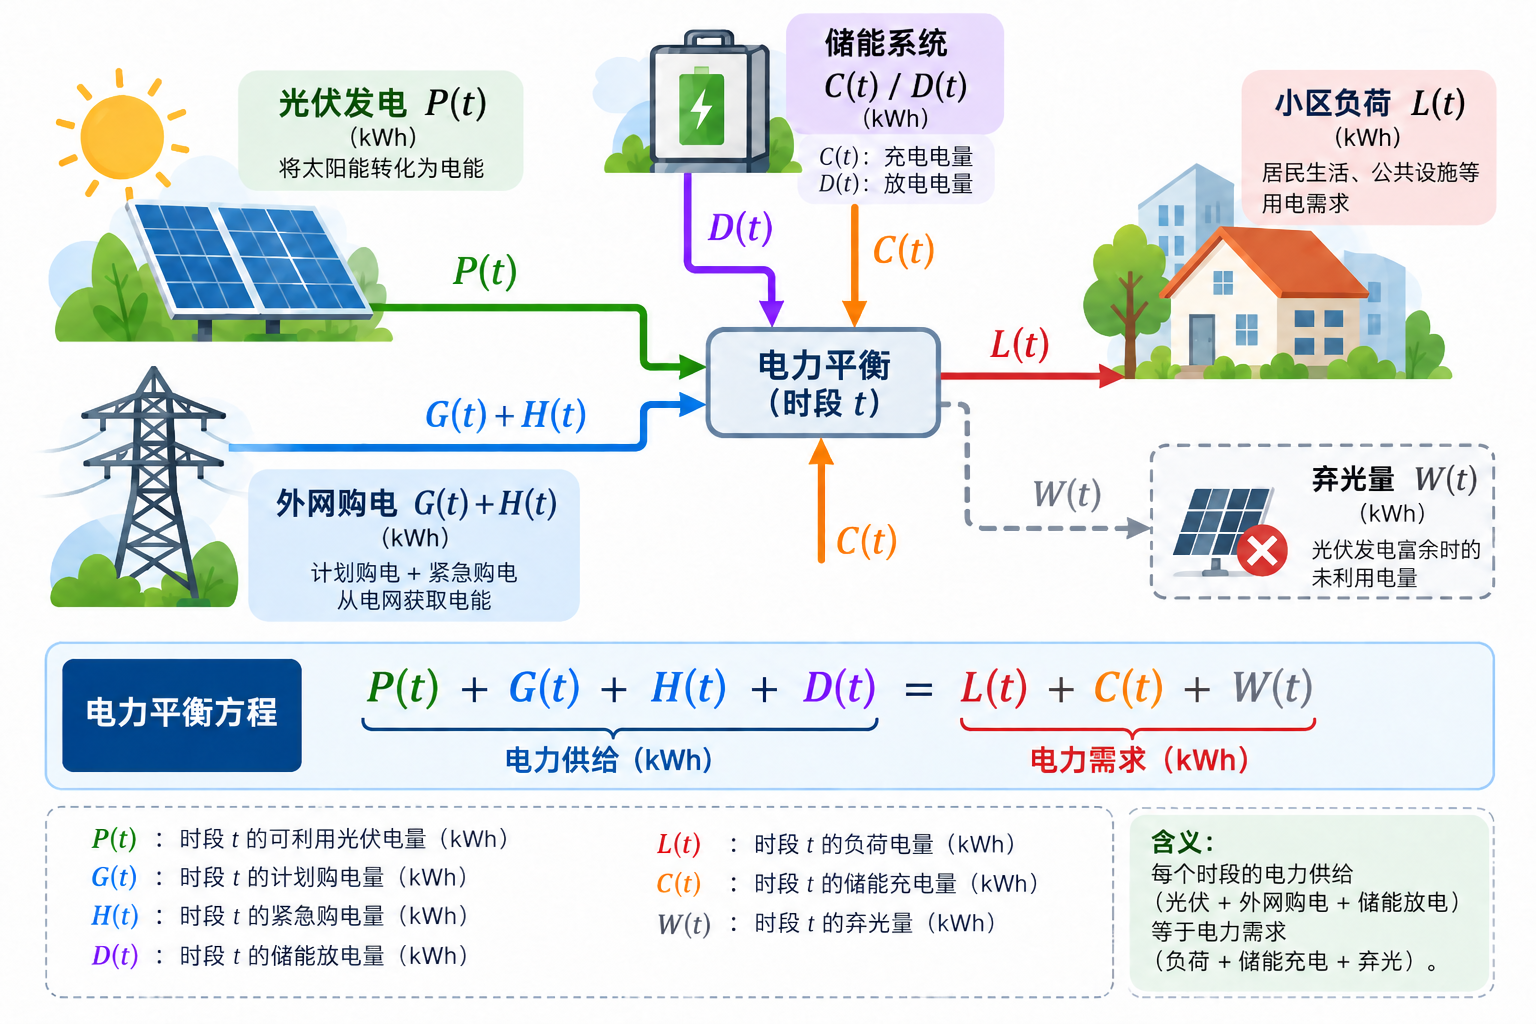
\includegraphics[width=0.96\textwidth]{../figures/电力平衡.png}
  \caption{贯穿全文的微网电力平衡关系}
  \label{fig:unified_power_balance}
\end{figure}

建模前需先锁定几处口径：10 分钟时刻标签是区间起点还是终点、90\% 是单程效率还是往返效率、问题三下调购电如何结算、问题四是否允许提前知道全天电价。这些口径直接决定结果的含义，本文在模型假设中逐条锁定基准并说明备选解释的影响，在对应小问内再结合模型交代其作用。总体技术路线如图~\ref{fig:roadmap} 所示：读取数据并统一量纲，建立公共调度内核，按各问特点扩展预测、场景或滚动机制，最后用当天实际值回放结算并校验。这样既保证模型结构一致，也便于把费用的变化归因到具体因素。

\begin{figure}[H]
  \centering
  \definecolor{cLvData}{HTML}{4A7BA7}%
  \definecolor{cLvCore}{HTML}{4C9279}%
  \definecolor{cLvSub}{HTML}{C08B45}%
  \definecolor{cLvChk}{HTML}{7E6BA8}%
  \resizebox{\textwidth}{!}{%
  \begin{tikzpicture}[
    font=\small,
    blk/.style={draw, rounded corners=2.5pt, align=center, inner sep=5pt,
                minimum height=9mm, line width=0.6pt},
    lv1/.style={blk, draw=cLvData, fill=cLvData!10},
    lv2/.style={blk, draw=cLvCore, fill=cLvCore!10},
    lv3/.style={blk, draw=cLvSub,  fill=cLvSub!10},
    lv4/.style={blk, draw=cLvChk,  fill=cLvChk!10},
    ar/.style={-{Stealth[length=2.4mm]}, semithick, draw=black!60},
  ]
    \node[lv1, text width=14.6cm] (data) at (0,0)
      {附件 1$\sim$4 数据读取与预处理：统一 144 个 10 分钟时段，功率 $\times\frac16\,\mathrm{h}$ 转换为电量};
    \node[lv2, text width=14.6cm] (core) at (0,-2.1)
      {公共调度内核：逐时段电力平衡 + 储能状态递推 + 充放电互斥 + 储电量与功率边界};
    \node[lv3, text width=3.3cm] (q1) at (-5.85,-4.9) {\textbf{问题一}\\确定性线性规划\\与互斥性核查};
    \node[lv3, text width=3.3cm] (q2) at (-1.95,-4.9) {\textbf{问题二}\\周期加权预测\\联合场景 MILP};
    \node[lv3, text width=3.3cm] (q3) at (1.95,-4.9)  {\textbf{问题三}\\官方光伏预报\\四时点滚动调整};
    \node[lv3, text width=3.3cm] (q4) at (5.85,-4.9)  {\textbf{问题四}\\波动电价预测\\四时点滚动调整};
    \node[lv4, text width=14.6cm] (settle) at (0,-7.7)
      {当天实际值回放结算 + 电力平衡、储能边界、充放电互斥与费用复算校验};
    \draw[ar] (data) -- (core);
    \draw[semithick] (-5.85,-3.4) -- (5.85,-3.4);
    \draw[ar] (core.south) -- (0,-3.4);
    \foreach \q in {q1,q2,q3,q4} { \draw[ar] (\q.north |- 0,-3.4) -- (\q.north); }
    \draw[semithick] (-5.85,-6.5) -- (5.85,-6.5);
    \foreach \q in {q1,q2,q3,q4} { \draw[ar] (\q.south) -- (\q.south |- 0,-6.5); }
    \draw[ar] (0,-6.5) -- (settle.north);
  \end{tikzpicture}}
  \caption{四问的统一技术路线}
  \label{fig:roadmap}
\end{figure}
